\section{The Finite State Machine}
The FSM manages the interactions between the CAPP and the host computer and it is responsible for orchestrating the individual CAPP operations necessary to implement complex arbitrary algorithms on the host computer.
It has numerous states, such as those for sending or receiving data, loading data into the CAPP, searching the memory (which in turn requires setting the comparand and mask) as well as reading the combined output. To implement the communication with the host computer we use base UART module provided in David Things' Github repository \cite{uart}. To reduce complexities and minimize our LUT-budget, we adopted the 48MHz clock speed used by the UART module throughout this project. 

\begin{figure}
  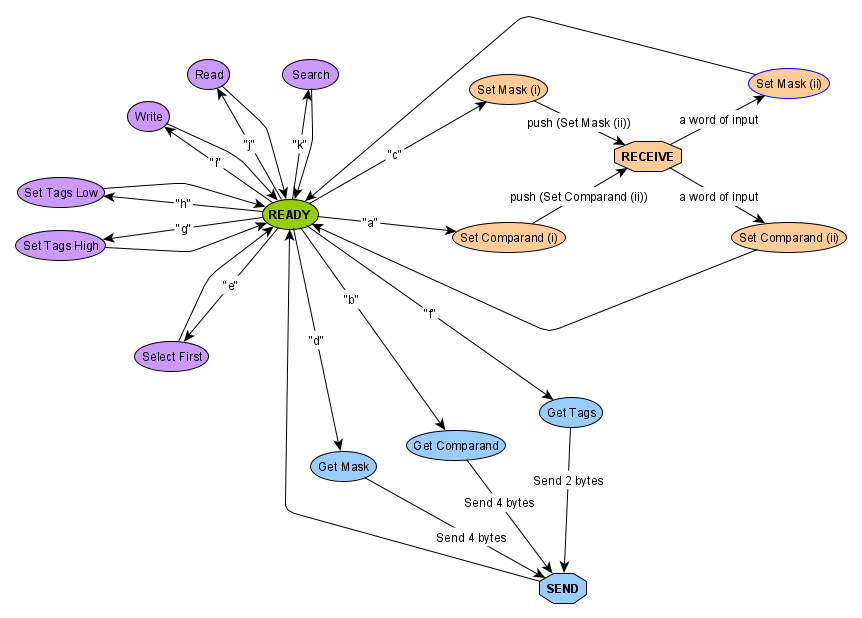
\includegraphics[height=6cm]{FPGA-CAPP_research_paper/images/protocol.png}
  \caption{Overview of the FSM underlying the CAPP-host protocol}
  \label{FSM_protocol}
\end{figure}

As shown in Figure \ref{FSM_protocol}, our FSM will typically break down a task into multiple short procedural tasks to reduce both magnitude and variance of the latency associated with each atomic state/task. In other words, we attempted to have a repertoire of tasks which all had (similarly) short latencies. Consequently, an overall task may necessitate several atomic states before returning the CAPP to its default ready state. 
For example, the operations for searching involve several steps, which are typically initiated by the Python "driver" and include:

\begin{itemize}
    \item Resetting the tags (set tags high, followed by set tags low)
    \item Setting the comparand 
    \item Setting the mask 
    \item Sending the search signal 
\end{itemize}

Notice that setting the comparand and mask require several clock cycles as the memory is based on 4-byte words and the CAPP can only send one byte per CAPP clock cycles. Furthermore, the FSM diagram shows a single RECEIVE state that can be used to receive both the comparand and the mask. Technically, in a formal FSM diagram, this should be represented by two distinct states, however, the Verilog code re-uses some logic when implementing these operations and we wanted the FSM-diagram to reflect this.

As seen above, resetting the tags is, in fact, a two step operations:

\begin{itemize}
    \item Set Tags High: change SET to high
    \item Set Tags Low: change SET to low
\end{itemize}
where SET refers to the SET line shown in Figure \ref{tag_registers}.

Some operations that appear to be atomic in Figure \ref{FSM_protocol} are in fact composed of multiple micro-steps, including an "IDLE" (delay) step. For example, the Search command is in fact composed of three micro-steps:

\begin{itemize}
    \item SEARCH\_1: 
        \begin{itemize}
            \item set SEARCH to high
            \item set delay to 5 clock cycles
        \end{itemize}
    \item IDLE:
        \begin{itemize}
            \item wait for duration of delay
            \item go to SEARCH\_2
        \end{itemize}
    \item SEARCH\_2: 
        \begin{itemize}
            \item set SEARCH to low
        \end{itemize}
\end{itemize}

where SEARCH refers to the "Perform Search" line in Figure \ref{search_circuit}. IDLE represents another case of a "shared" micro-step which is reused by two commands (as was the case with RECEIVE). Though it is not represented in Figure \ref{FSM_protocol} (in the interest of clarity), IDLE is in fact used by both the Search and Select commands.
